\section{Resolución Problema 6}
\subsection{Problema:}
Dada una tabla de verdad de $n$ bits generar la expresión booleana que genere de manera fidedigna las salidas de esta tabla.

\subsection{\textbf{Descripción del problema:}}
Se dispone de una tabla que exhibe múltiples combinaciones de unos y ceros que se forman debido a la naturaleza de la representación de las entradas binarias, junto con los resultados deseados asociados a cada combinación. \\
La tarea consiste en hallar una expresión booleana que describa de manera lógica estas relaciones.


\subsection{\textbf{Definición de solución:}}
Para resolver este problema, se adopta la técnica conocida como "Suma de Productos" (Sum-Of-Products, o SOP en inglés). Esta metodología implica identificar las combinaciones específicas para las cuales la salida es igual a 1. Posteriormente, estas condiciones se combinan utilizando operaciones lógicas AND, incluyendo la posibilidad de la operación NOT para algunas variables. \\
Estos conjuntos de condiciones AND, que pueden incluir negaciones (NOT), se consolidan mediante la operación lógica OR. El resultado final es una expresión booleana que representa de manera clara y sencilla la lógica detrás de la tabla de verdad.\\ 

\begin{figure}[h!]
    \centering
    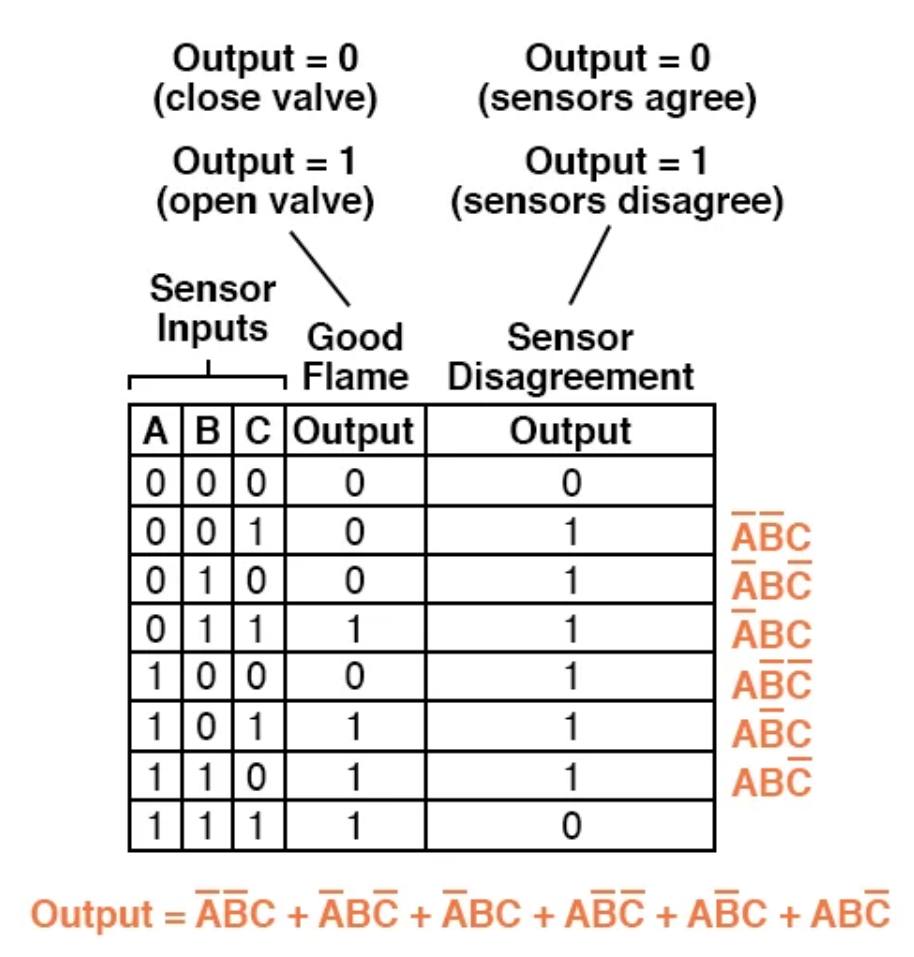
\includegraphics[width=0.7\linewidth]{./latex-imágenes/truth-table.png}
    \caption{Suma de productos para una tabla de verdad}
    \label{fig:enter-label}
\end{figure}
La siguiente notación se relaciona directamente con la técnica de la Suma de Productos (SOP) mencionada previamente.\\
\[ F(A, B, C, ...) = \Sigma(m_i) \]
Donde:
\begin{itemize}

  \item[{\ieeeguilsinglright}] {\it \(\Sigma(m_i)\):} Indica que se está sumando sobre los términos \(m_i\), donde \(i\) representa los índices que van desde el valor inicial hasta el valor final.

  \item[{\ieeeguilsinglright}] {\it \(m_i\):} Cada término \(m_i\) es un producto que representa una combinación específica de las variables \(A, B, C, ...\) y sus negaciones.
\end{itemize}

Se centra únicamente en las salidas con valor 1 porque estas representan los casos en los que la función booleana es verdadera o activa, si la salida es 0 para una combinación particular de entradas, ese caso no contribuirá al término de suma de productos


\subsection{\textbf{Diseño de la Solución:}}

\begin{itemize}
    \item[{\ieeeguilsinglright}] {\it Entrada de Datos:}
        Se solicita la cantidad de bits (\(n\)) y las posiciones de salidas activas.
        
    \item[{\ieeeguilsinglright}] {\it Generación de la Tabla de Verdad:}
        Se crea la tabla de verdad con todas las combinaciones posibles de\(n\) bits.

    \item[{\ieeeguilsinglright}] {\it Identificación de Combinaciones Activas:}
        Se determinan las combinaciones de entradas que resultan en salidas activas (1).

    \item[{\ieeeguilsinglright}] {\it Generación de Términos de Producto:}
        Para cada combinación activa, se crea un producto con la multiplicación binaria (AND).

    \item[{\ieeeguilsinglright}] {\it Construcción de la Expresión Booleana:}
        Los producto se combinan con la suma de todos estos (OR).

    \item[{\ieeeguilsinglright}] {\it Presentación de la Expresión:}
         Se muestra la expresión booleana final.        
\end{itemize}
\newpage

\subsection{\textbf{Desarrollo de la solución:}}

Se solicita al usuario la cantidad de bits y las posiciones de las salidas activas, con esto de calcula la cantidad de columnas y filas para la tabla desde el método(\texttt{main}).
\begin{javaCode}
Scanner entradaDatos = new Scanner(System.in);
    //Entrada de datos cantidad de bits 
    System.out.print("Ingrese la cantidad de bits: ");
    int numBits = entradaDatos.nextInt();
    entradaDatos.nextLine();
    
    //Entrada de salidas con valor 1
    int numSalidas = (int)Math.pow(2, numBits);
    int[][] tabla = new int[numSalidas][numBits+1];
    System.out.print("Ingrese las salidas que son 1 sepadados por comas ("+1+"-"+numSalidas+"): ");
    String[] salidas = entradaDatos.nextLine().split(",");
    entradaDatos.close();//cerrar captura de datos
\end{javaCode}

La función \texttt{llenarTabla} llena una matriz con todas las combinaciones posibles de bits y asigna los valores de salida correspondientes y retorna la matriz que representa la tabla con los valores corrspondientes.
\begin{javaCode}
    public static int[][] llenarTabla(int[][] tabla, int numBits, String[] salidas) {
    //...codigo restante
    return tabla;
    }
\end{javaCode}
   \begin{itemize}
       \item[{\ieeeguilsinglright}] {\it } Convierte las posiciones de salida activas en un arreglo tipo entero para su fácil manejo.
   \begin{javaCode}
    int[] salidasInt = new int[salidas.length];
    for (int i = 0; i < salidasInt.length; i++) {
        salidasInt[i] = Integer.parseInt(salidas[i])-1;
    }
    Arrays.sort(salidasInt);
   \end{javaCode}
       
       \item[{\ieeeguilsinglright}] {\it }  Utiliza bucles \texttt{for} para asignar todas las combinaciones de bits y asigna las salidas activas haciendo uso de condicionales.
    \begin{javaCode}
    /Llenar las combinaciones
    for (int i = 0; i < tabla.length; i++) {
        for (int j = 0; j < numBits; j++) {
            int division = i / ((int) Math.pow(2, j));
            int valorPosicion = division % 2;
            tabla[i][(numBits)-1-j] = (valorPosicion == 0)   ?   1 : 0 ;
        }
    }
    // LLenar las salidas de la tabla
    for (int i = 0; i < tabla.length; i++) {
        if (Arrays.binarySearch(salidasInt, i) >= 0) {
            tabla[i][numBits] = 1;
        } else {
            tabla[i][numBits] = 0;
        }
    }
    \end{javaCode}

   \end{itemize}


Las combinaciones activas (salida igual a 1) se identifican y se almacenan en una matriz auxiliar.
\begin{javaCode}
//Obtener las filas con salidas de valor 1
String[][] salidasUno = new String[salidas.length][filas-1];
int indice = 0;
for (int i = 0; i < filas; i++) {
    if (tablaDeVerdad[i][columnas-1] == 1) {
        for (int j = 0; j < columnas-1; j++) {
            salidasUno[indice][j] = 
            Integer.toString(tablaDeVerdad[i][j]);
        }
        indice++;
    }
}
\end{javaCode}

Se asigna la letra correspondiente y se crea un producto para cada combinación activa utilizando la multiplicación binaria.
\begin{javaCode}
//Cambiar valores por la letra correspondiente
    for (String[] salidasUno1 : salidasUno) {
        for (int j = 0; j < columnas-1; j++) {
            if ("0".equals(salidasUno1[j])) {
                salidasUno1[j] = "-"+preposiciones.charAt(j);
            } else {
                salidasUno1[j] = ""+preposiciones.charAt(j);
            }
        }
    }
\end{javaCode}

Se construye la expresión booleana combinando los términos de producto con la suma de todos ellos.
\begin{javaCode}
//Concatear arreglo en una cadena
for (int i = 0; i < salidasUno.length; i++) {
    for (int j = 0; j < columnas-1; j++) {
        expresion += salidasUno[i][j];
    }
    if (i != salidasUno.length-1) {
        expresion += " + ";
    }
}
\end{javaCode}
La función \texttt{imprimirTabla} imprime la tabla de verdad en la consola con colores para una mejor visualización iterando por cada  encabezado y elementos de la matriz.
\begin{javaCode}
//Datos
    int filas = tablaDeVerdad.length;
    int columnas = tablaDeVerdad[1].length;
    String preposiciones= "ABCDEFGHIJKLMNOPQRSTUVWXYZ";
    String[] colores = {
        "\u001B[31m", // rojo
        "\u001B[34m", // azul
        "\u001B[32m", // verde
        "\u001B[35m", // morado
        "\u001B[33m", // amarillo
        "\u001B[36m", // cian
    };
\end{javaCode}
\newpage
\begin{itemize}
       \item[{\ieeeguilsinglright}] {\it } Se itera por los encabezados correspondientes
\begin{javaCode}    
    //Imprimir la tabla
    System.out.println("\nLa tabla de verdad es:");
    // Encabezados
    System.out.print("     ");
    for (int i = 0; i <= columnas-1; i++) {
        if (i == columnas-1) {
            System.out.print(colores[i] + "Salida");
        }else{
            System.out.print(colores[i] + preposiciones.charAt(i) + "  ");
        }
    }
    System.out.println();
\end{javaCode}
    \item[{\ieeeguilsinglright}] {\it } Se itera por los el contenido de la tabla
\begin{javaCode}
    //Combinaciones de la tabla
    for (int i = 0; i < filas; i++) {
        if (i<9) {
            System.out.print(" ");
        }
        System.out.print(i+1+"| ");
        for (int j = 0; j <= columnas-1; j++) {
            System.out.print(" " +colores[j] + tablaDeVerdad[i][j] + " ");
        }
        System.out.println();
    }
\end{javaCode}
\end{itemize}


En el método principal (\texttt{main}) se genera la tabla de verdad, la imprime y muestra la expresión booleana resultante.
\begin{javaCode}
public static void main(String[] args) {
    //resto del codigo
    /*PROCESOS*/
    tabla = llenarTabla(tabla, numBits,salidas);//Llenar tabla
    
    imprimirTabla(tabla);//imprimimos la tabla generada
    
    System.out.println("\nExpresion booleana: ");
    String expresion = generarExpresionBooleana(salidas, tabla);//Generar expresion booleana
    System.out.println(expresion+"\n");//Mostrar la expresion
}
\end{javaCode}

\subsection{\textbf{Depuración y pruebas:}}

\begin{table}[h]
\centering
\begin{tabular}{|c|c|c|c|c|}
\hline
\textbf{Nº} & \textbf{A} & \textbf{B} & \textbf{C} & \textbf{Salida} \\
\hline
1 & 1 & 1 & 1 & 1 \\
2 & 1 & 1 & 0 & 0 \\
3 & 1 & 0 & 1 & 0 \\
4 & 1 & 0 & 0 & 0 \\
5 & 0 & 1 & 1 & 0 \\
6 & 0 & 1 & 0 & 1 \\
7 & 0 & 0 & 1 & 0 \\
8 & 0 & 0 & 0 & 0 \\
\hline
\end{tabular}
\caption{Tabla de verdad 1}
Expresión booleana: $ABC + A'BC'$
\end{table}
\newpage
\begin{table}[h]
\centering
\begin{tabular}{|c|c|c|c|}
\hline
\textbf{Nº} & \textbf{A} & \textbf{B} & \textbf{Salida} \\
\hline
1 & 1 & 1 & 1 \\
2 & 1 & 0 & 1 \\
3 & 0 & 1 & 0 \\
4 & 0 & 0 & 0 \\
\hline
\end{tabular}
\caption{Tabla de verdad 2}
Expresión booleana: $AB + AB'$
\end{table}
